\chapter{Implementierung}
\label{ch:implementation}

\section{Architektur des Monorepos und Shared Logic}
\label{s:impl-monorepo}

Das Experiment ist als npm-Workspace-Monorepo aufgebaut, um sicherzustellen, dass beide Framework-Anwendungen identische Eingabedaten aus demselben Paket \code{@benchmark/shared-logic} erhalten (vgl.~\cref{sss:mock-engine-validity}). In der zentralen \texttt{package.json} sind vier Pakete deklariert: \code{@benchmark/shared-logic}, \texttt{react-app}, \texttt{svelte-app} und \code{@benchmark/runner}. npm löst Abhängigkeiten zwischen diesen Paketen lokal auf, ohne dass ein separater Paketregistrierungs-Schritt erforderlich ist. Beide Framework-Anwendungen nutzen \code{@benchmark/shared-logic} als direkte Abhängigkeit. Während der Installation bindet npm das Paket über einen Symlink im jeweiligen \texttt{node\_modules}-Verzeichnis ein \cite{npm-workspaces-2026}; dadurch greifen beide Anwendungen auf dieselbe versionierte Implementierung zu. Abbildung~\ref{fig:diagram-5-1} veranschaulicht die Struktur der Pakete und ihre Beziehungen.

\begin{figure}[htbp]
  \centering
  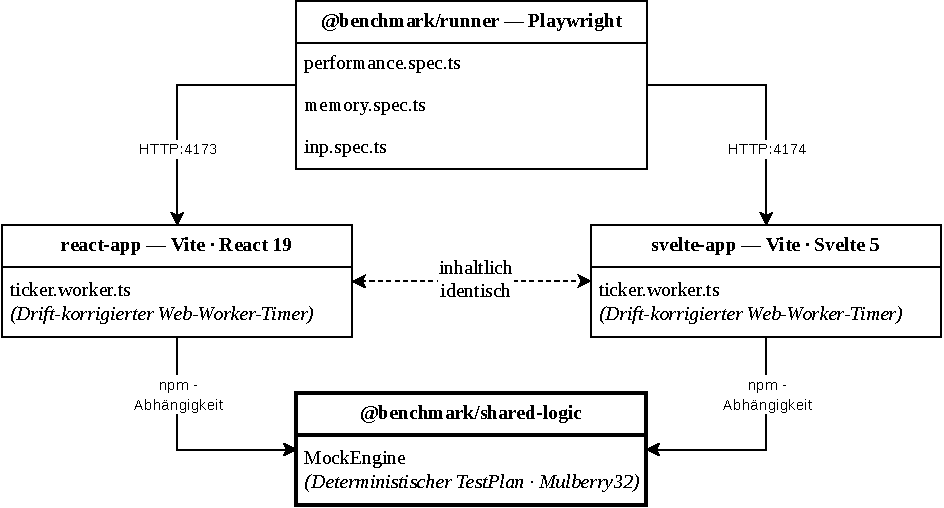
\includegraphics[width=\textwidth]{bilder/diagram_5_1.pdf}
  \caption{Paketstruktur und Abhängigkeitsbeziehungen des npm-Workspace-Monorepos.}
  \label{fig:diagram-5-1}
\end{figure}

\subsection{Das Paket \texttt{@benchmark/shared-logic}}
\label{ss:impl-shared-logic}

Das Paket \texttt{@benchmark/shared-logic} ist als reines TypeScript-Paket ohne Laufzeitabhängigkeiten implementiert; die Kompilierung erfolgt einmalig mit \texttt{tsc}.

\subsection{Datenmodell: Interfaces \texttt{GridItem}, \texttt{TickMutation} und \texttt{TestPlan}}
\label{ss:impl-interfaces}

Das Paket exportiert drei TypeScript-Interfaces, die das Datenmodell beider Anwendungen beschreiben (siehe \cref{lst:interfaces} im Anhang). \texttt{GridItem} repräsentiert eine einzelne Zelle des Grids mit eindeutiger numerischer ID sowie dem aktuellen Anzeigewert. \texttt{TickMutation} beschreibt eine Zustandsänderung einer einzelnen Zelle und spezifiziert deren ID sowie den zugehörigen Folgewert. \texttt{TestPlan} fasst den vollständigen Ablauf eines Szenarios zusammen: \texttt{initialState} enthält den Ausgangszustand aller Zellen, \texttt{ticks} ist ein zweidimensionales Array, dessen äußere Dimension die zeitliche Abfolge der Ticks beschreibt, während die innere Dimension die Zellen angibt, die pro Tick gleichzeitig aktualisiert werden. Der \texttt{TestPlan} entsteht einmalig vor dem ersten Render und bleibt anschließend unverändert (vgl. \cref{sss:mock-engine-validity}).

\subsection{Implementierung der \texttt{MockEngine}}
\label{ss:impl-mockengine}

Die Klasse \texttt{MockEngine} stellt die Methode \texttt{generateTestPlan(gridSize, tickCount, mutationRate, seed\,=\,123)} bereit. Zur Erzeugung deterministischer Zufallswerte kommt der Pseudozufallszahlengenerator Mulberry32 zum Einsatz \cite{ettinger-mulberry32-2017}, da \texttt{Math.random()} keine standardisierte Seed-Initialisierung bietet. Bei gleichem Seed liefert Mulberry32 reproduzierbare Float-Werte im Intervall $[0,1)$. Die Umsetzung auf Basis von 32-Bit-Ganzzahlarithmetik verursacht keinen messbaren Mehraufwand im Benchmark. Die Methode \texttt{generateTestPlan} durchläuft zwei Phasen. In der ersten Phase wird \texttt{initialState} befüllt: Für jede der \texttt{gridSize} Zellen erzeugt Mulberry32 einen Startwert im Bereich $[0, 100)$. Gleichzeitig speichert \texttt{currentValues} in einem Shadow-Array gleicher Länge die aktuellen Zellwerte, die in der zweiten Phase für die Bailout-Guard-Prüfung benötigt werden. In der zweiten Phase entstehen \texttt{tickCount} Tick-Einträge. Die Zahl der je Iteration zu mutierenden Zellen ergibt sich aus $\lceil \mathtt{gridSize} \cdot \mathtt{mutationRate} \rceil$. Die Bestimmung der Indizes erfolgt zufällig und ohne Zurücklegen (vgl. \cref{ss:scenario-a}); hierfür dient ein vorab angelegtes Array aller Zell-Indizes der Länge \texttt{gridSize}, das über alle Ticks hinweg wiederverwendet wird. In jeder Iteration werden nur die ersten \texttt{mutationCount} Positionen des Arrays durch gezielte Tauschoperationen neu angeordnet. Dabei entstehen genau \texttt{mutationCount} eindeutige Indizes ohne Duplikate. Im Vergleich zu einem vollständigen Shuffle mit $O(n)$ reduziert sich der Aufwand je Iteration auf $O(\mathtt{mutationCount})$ \cite{knuth-taocp2-1998}; die Wiederverwendung des Pools vermeidet zudem Heap-Allokationen pro Tick.
Für jeden selektierten Index stellt der Bailout-Guard (vgl. \cref{lst:bailout} im Anhang) sicher, dass der generierte Folgewert nicht mit dem gespeicherten Vorgänger übereinstimmt. Der neue Wert aktualisiert \texttt{currentValues} und gelangt zusammen mit der ID als \texttt{TickMutation} in das entsprechende Tick-Array.

\subsection{Der drift-korrigierte Web-Worker-Timer (\texttt{ticker.worker.ts})}
\label{ss:impl-worker}

Beide Framework-Anwendungen verwenden eine inhaltlich identische Datei \code{ticker.worker.ts}, die als separater Web Worker läuft. Nach dem Empfang einer Startnachricht mit dem gewünschten Tick-Intervall startet er einen Tick-Scheduler, der Drift durch kumulativen Zeitabgleich korrigiert \cite{mills-rfc5905-2010} (vollständiger Code: \cref{lst:worker} im Anhang). Bei jedem Aufruf von \texttt{scheduleNextTick} findet ein Abgleich der realen Ausführungszeit mit \texttt{expectedTime} statt. Die dabei gemessene Abweichung (\texttt{drift}) wird vom nächsten Delay abgezogen, sodass Verspätungen einzelner Ticks in nachfolgenden Intervallen kompensiert werden. Der Worker sendet lediglich ein Zeitsignal. Die eigentlichen Mutationsdaten empfangen die Anwendungen über einen internen Tick-Zähler aus dem vorab berechneten \texttt{TestPlan}. Durch die Ausführung des Workers in einem eigenen Agent-Thread mit separater Event-Loop bleibt die Tick-Frequenz unabhängig von der Rendering-Last des Main Threads \cite{whatwg-html-2026} (vgl. \cref{sss:disturbances}).

\section{Technische Umsetzung der React-Referenzanwendung}
\label{s:impl-react}

Die React-Referenzanwendung ist als Vite-Projekt mit React~19 umgesetzt und besteht aus drei Ebenen: \texttt{App.tsx} bildet den Einstiegspunkt der Anwendung, \texttt{Grid.tsx} übernimmt die Anordnung der Inhalte und \texttt{Cell.tsx} stellt die einzelnen Zellen dar. Dieser Aufbau erfüllt die in \cref{sss:parity} formulierte Anforderung der strukturellen Vergleichbarkeit. Gleichzeitig dient die Anwendung als Grundlage zur Untersuchung des React-Compilers in einer typischen Komponentenstruktur mit geringer Verschachtelungstiefe.

\subsection{Komponentenstruktur und Prop-Weitergabe}
\label{ss:impl-react-components}

Der vollständige \texttt{TestPlan} entsteht in \texttt{App.tsx} bereits auf Modulebene vor der Definition der Komponenten (vgl. \cref{sss:mock-engine-validity}), sodass die Berechnung nur einmal beim Laden des Bundles erfolgt und nicht bei jedem Render-Aufruf. Der Initialzustand des Grids liegt in einem \texttt{useState}-Array vom Typ \texttt{GridItem[]} vor. Darüber hinaus existieren zwei weitere \texttt{useState}-Felder für den Ablaufstatus (\texttt{phase}) und die UI-Fortschrittsanzeige (\texttt{tickCount}). \texttt{App.tsx} gibt das Array als \texttt{items}-Prop an \texttt{Grid.tsx} weiter, das lediglich die Layoutstruktur bereitstellt (vollständiger Komponentencode: \cref{lst:react-grid} im Anhang). 
\noindent\texttt{Grid.tsx} übergibt an \texttt{Cell} den Integer \texttt{value} anstelle des gesamten \texttt{GridItem}-Objekts. Dadurch kann der React-Compiler die Komponente memoisieren und die erneute Ausführung der Renderfunktion vermeiden, solange sich der Wert nicht ändert. Lokale Zustandsänderungen führen weiterhin zu regulären Re-Renders.
Zudem beschränkt sich der Prop-Vergleich des React~Compilers auf einen einfachen Integer-Gleichheitscheck (\texttt{===}), was die strukturelle Vergleichbarkeit mit der Svelte-Implementierung sicherstellt (vgl.~\cref{sss:parity}). \texttt{Cell.tsx} repräsentiert die einzelnen Zellen des Grids. Die Komponente rechnet den übergebenen Wert zur visuellen Hervorhebung in eine Farbe im Farbmodell Hue, Saturation, Lightness (HSL) um. Für den INP-Trigger (vgl.~\cref{sss:inp-trigger}) verwaltet die Komponente zusätzlich einen lokalen \texttt{clicked}-Zustand.

\subsection{Unveränderliche Referenzaktualisierung im Tick-Handler}
\label{ss:impl-react-update}

React erkennt Zustandsänderungen anhand von Objektreferenzen (\cref{ss:vdom}). Der Tick-Handler in \texttt{App.tsx} nutzt dieses Prinzip (vollständiger Code: \cref{lst:react-update} im Anhang): Der Spread-Operator \texttt{[...prev]} erzeugt zunächst eine flache Kopie des Arrays. Für jede der $\lceil n \cdot 0{,}05 \rceil$ mutierten Zellen (vgl.~\cref{ss:scenario-a}) erfolgt anschließend das Einfügen eines neuen \texttt{\{id, value\}}-Objekts an der jeweiligen Position. Alle übrigen Positionen behalten ihre ursprünglichen Objektreferenzen. Diese Eigenschaft ist entscheidend für die Korrektheit der Messung: Da \texttt{Grid} das gesamte \texttt{items}-Array als Prop erhält, löst jede Tick-Mutation ein erneutes Rendering aus. Anschließend vergleicht der React-Compiler für jede \texttt{Cell} den aktuellen \texttt{value}-Prop mit dem zuvor gespeicherten Wert (\texttt{===}) \cite{react_reconcillation_2024}. Nur bei einer Änderung führt die jeweilige Zelle ihre Renderfunktion erneut aus. Abbildung \ref{fig:diagram-5-2-3} zeigt diesen Mechanismus im Vergleich zum Ansatz der direkten Zustandsänderung in Svelte~5. Die flache Kopie des Arrays wirkt sich auch auf die Speicheranalyse aus (\cref{sss:quantitative-heap}): Pro Tick entstehen $\lceil n \cdot 0{,}05 \rceil$ neue \texttt{GridItem}-Objekte sowie ein neues Array der Länge~$n$. Die ersetzten Objekte werden zu Garbage-Collection-Kandidaten.
\begin{figure}[htbp]
  \centering
  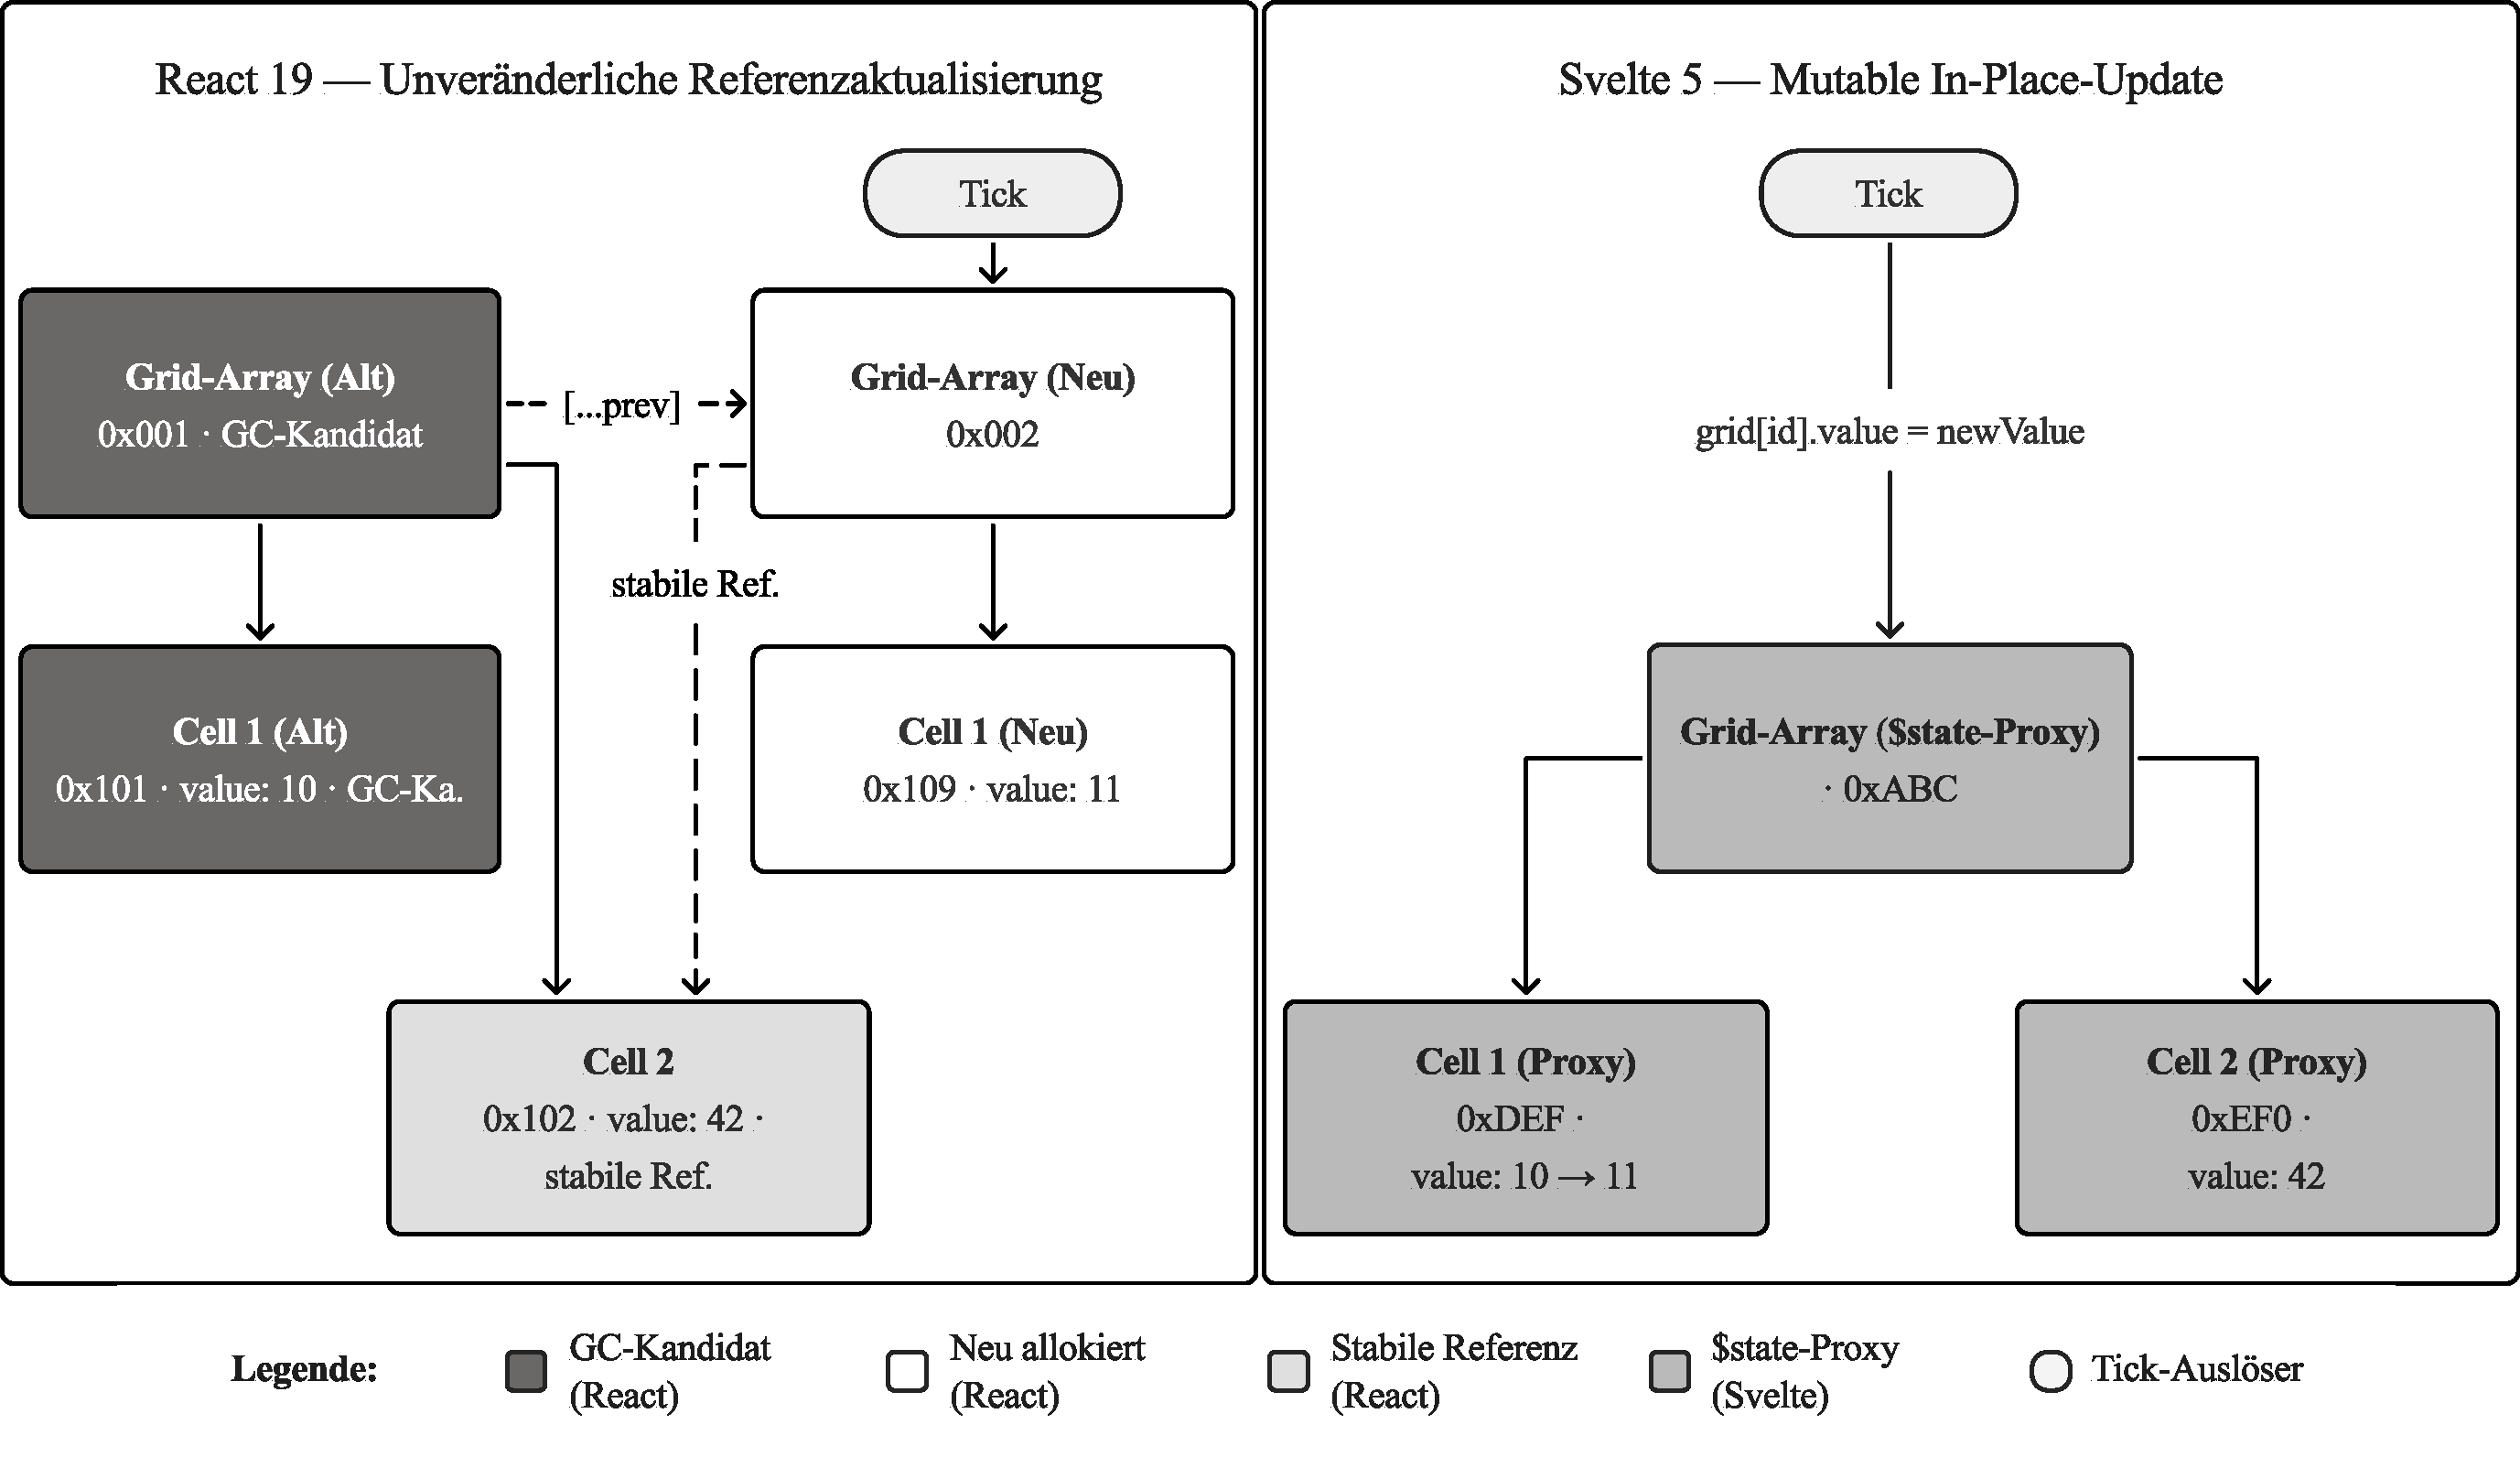
\includegraphics{bilder/diagram_5_2_3.pdf}
  \caption[Gegenüberstellung der Update-Strategien React~19 und Svelte~5]{Gegenüberstellung der Update-Strategien: React~19 arbeitet mit der Erzeugung neuer Heap-Objekte bei jeder Änderung (dunkelgrau markiert als Garbage-Collection-Kandidaten), während Svelte~5 bestehende Signal-Objekte direkt aktualisiert und so zusätzliche Speicherallokationen weitgehend vermeidet (Eigene Darstellung, KI-unterstützt).}
  \label{fig:diagram-5-2-3}
\end{figure}

\subsection{Steuerung durch den Web Worker und Benchmark-Ablauf}
\label{ss:impl-react-worker}

\texttt{App.tsx} instanziiert den Web Worker (\cref{ss:impl-worker}) in einem \texttt{useEffect}-Hook mit leerer Abhängigkeitsliste (\texttt{[]}), sodass die Initialisierung nur einmal nach dem ersten Rendern erfolgt. Zusätzlich registriert der Hook einen \texttt{'benchmark-start'}-Event-Listener auf \texttt{window}. Die vollständige Startlogik ist in \cref{lst:react-lifecycle} im Anhang abgebildet. Das Flag \texttt{IS\_BENCHMARK\_MODE} ist \texttt{true}, sobald der Query-Parameter \texttt{gridSize} in der URL vorhanden ist; andernfalls löst die Anwendung das Ereignis selbst aus und startet unmittelbar. Das \texttt{data-testid}-Attribut des Root-Elements wechselt von \texttt{'benchmark-ready'} auf \texttt{'benchmark-done'}, sobald der Worker beendet wurde und \texttt{setPhase('done')} den zugehörigen React-Re-Render ausgelöst hat (vgl.~\cref{sss:lifecycle}).

\subsection{Integration des React Compilers}
\label{ss:impl-react-compiler}

Die Datei \texttt{vite.config.ts} bindet den React-Compiler als Babel-Plugin in die Build-Pipeline ein (vollständige Konfiguration: \cref{lst:react-compiler-config} im Anhang). Das Plugin \texttt{@vitejs/plugin-react} übernimmt die Standard-Umwandlung von JavaScript XML (JSX), während \texttt{@rolldown/plugin-babel} die anschließende Compiler-Umwandlung ausführt. Die Funktion \texttt{reactCompilerPreset()} bindet \texttt{babel-plugin-react-compiler} als Preset ein und aktiviert es in der in \cref{ss:software-versions} festgelegten Version~1.0.0. Der Compiler analysiert jede Komponente statisch auf Seiteneffekte und veränderte Props. Komponenten ohne solche Eigenschaften werden automatisch memoisiert, sodass das Ergebnis des letzten Renderns zwischengespeichert und eine erneute Ausführung bei unveränderten Eingaben verhindert wird \cite{react_compiler_2025}. Ob der Compiler korrekt aktiv ist, lässt sich auf zwei Ebenen überprüfen. Auf Build-Ebene enthält das erzeugte JavaScript-Bundle typische Compiler-Artefakte, darunter direkte Aufrufe der internen Funktion \texttt{\_c} sowie Zugriffe auf ein Cache-Array, das durch das Symbol \texttt{\$} dargestellt wird. Auf Laufzeitebene kennzeichnet der React DevTools Profiler optimierte Komponenten mit der Annotation \guillemotleft{}Memo\guillemotright{}, wobei ein zusätzliches Sparkle-Symbol anzeigt, dass die Memoisierung automatisch durch den Compiler erfolgte \cite{gsathya-compiler-2024}. Beide Indikatoren sind im vorliegenden Setup erfüllt: Die Komponenten \texttt{App}, \texttt{Grid} und \texttt{Cell} wurden vollständig optimiert. Wie in \cref{sss:forbidden-optimizations} dargelegt, enthält der Quellcode keine manuellen Optimierungen mittels \texttt{React.memo}, \texttt{useMemo} oder \texttt{useCallback}. Zudem hat der \texttt{<StrictMode>}-Wrapper in \texttt{main.tsx} im Production-Build keine Auswirkungen und beeinflusst die Messergebnisse daher nicht (vgl.~\cref{sss:production-build}).

\section{Technische Umsetzung der Svelte-Referenzanwendung}
\label{s:impl-svelte}

Die Umsetzung in Svelte folgt der in \cref{s:impl-react} beschriebenen Dreistufenarchitektur (\texttt{App.svelte}, \texttt{Grid.svelte}, \texttt{Cell.svelte}) und stellt damit die strukturelle Vergleichbarkeit sicher (vgl.~\cref{sss:parity}). Svelte-4-Elemente wie (\texttt{export let}, reaktive Statements \texttt{\$:} und Svelte Stores) kommen nicht zum Einsatz; alle Dateien verwenden ausschließlich die Runes-Syntax von Svelte~5 (vgl.~\cref{sss:forbidden-optimizations}).

\subsection{Komponentenstruktur und Prop-Weitergabe}
\label{ss:impl-svelte-components}

In Svelte~5 gibt es innerhalb einer \texttt{.svelte}-Datei zwei Script-Blöcke: \texttt{<script module>} enthält Code auf Modulebene, der beim Laden genau einmal ausgeführt wird; \texttt{<script>} umfasst instanzbezogenen Code, der bei jedem Mount einer Komponente läuft. In \texttt{App.svelte} kommt diese Trennung gezielt zum Einsatz: Der \texttt{TestPlan} entsteht im \texttt{<script module>}-Block (vgl.~\cref{sss:mock-engine-validity} und \cref{lst:svelte-module} im Anhang), wodurch die Berechnung nicht bei jedem Rendern erneut erfolgt. Das Grid ist im komponentenbezogenen \texttt{<script>}-Block als \texttt{\$state}-Array deklariert (vgl. \cref{lst:svelte-state} im Anhang). Der Spread-Operator \texttt{\{...item\}} erzeugt für jedes \texttt{GridItem}-Objekt eine flache Kopie. Dadurch arbeitet die Anwendung mit eigenen, veränderbaren Instanzen, während der \texttt{TestPlan} selbst unverändert bleibt. \texttt{\$state()} erlaubt es, Änderungen an einzelnen Eigenschaften zur Laufzeit gezielt nachzuverfolgen (vgl.~\cref{sss:finegraned-reactivity}). Die Prop-Weitergabe an \texttt{Grid.svelte} und \texttt{Cell.svelte} erfolgt über die Rune \texttt{\$props()} (vgl. \cref{lst:svelte-props} im Anhang). \texttt{Grid.svelte} iteriert mit einem schlüsselbasierten \texttt{\{\#each\}}-Block und übergibt ausschließlich den primitiven \texttt{value}-Integer an \texttt{Cell}. \texttt{Cell.svelte} verwaltet intern einen \texttt{clicked}-Zustand als \texttt{\$state}. Beide Entscheidungen sind strukturell identisch mit der React-Implementierung (vgl.~\cref{ss:impl-react-components}).

\subsection{Direkte Zustandsmutation im Tick-Handler}
\label{ss:impl-svelte-update}

Der Unterschied liegt in der Art der Zustandsänderung. Anstatt bei jeder Änderung ein neues Array zu erzeugen (vgl.~\cref{ss:impl-react-update}), mutiert Svelte~5 die vorhandenen Objekte direkt (vollständiger Tick-Handler: \cref{lst:svelte-update} im Anhang). Der \texttt{\$state}-Proxy erkennt und verarbeitet die Zuweisung \texttt{grid[id].value = newValue}. Der \texttt{\{\#each\}}-Block in \texttt{Grid.svelte} generiert zur Laufzeit pro Iteration eine feingranulare reaktive Bindung auf \texttt{item.value}. \texttt{Cell.svelte} selbst enthält dabei keine eigene Reaktivitätslogik, sondern empfängt lediglich den aktualisierten primitiven Wert als Prop. Eine Property-Änderung aktualisiert ausschließlich die betroffene \texttt{Cell}, ohne dass das Array kopiert wird, neue Objektreferenzen erzeugt werden oder der gesamte Komponentenbaum durchlaufen wird (vgl.~\cref{sss:finegraned-reactivity}), wodurch die Referenzen auf die einzelnen Objekte in \texttt{grid} während des gesamten Benchmark-Verlaufs stabil bleiben. Reacts \texttt{setGrid}-Aufruf erzeugt hingegen pro Tick neue Objekte und eine neue Array-Instanz (vgl.~\cref{ss:impl-react-update}). Abbildung~\ref{fig:diagram-5-2-3} zeigt diesen Kontrast: React hinterlässt Garbage-Collection-Kandidaten, während Svelte den Heap-Speicherbedarf stabil hält. Dieser strukturelle Unterschied gilt als erwartete Ursache des in Hypothese H3 untersuchten JS-Heap-Deltas (vgl.~\cref{ss:hypotheses}).

\subsection{Steuerung durch den Web Worker und Benchmark-Ablauf}
\label{ss:impl-svelte-worker}

Ein \texttt{\$effect}-Block übernimmt die Instanziierung des Workers (vollständige Implementierung: \cref{lst:svelte-effect} im Anhang). Anders als \texttt{useEffect} in React benötigt \texttt{\$effect} kein Dependency-Array \cite{react_introduction, svelte_migration}, da reaktive Abhängigkeiten automatisch ermittelt werden (vgl.~\cref{ss:svelte-reactivity}). Da dieser Effekt keinen reaktiven State verwendet, besitzt er keine Abhängigkeiten und entspricht somit \texttt{useEffect(fn, [])}; der Rückgabewert ist eine Cleanup-Funktion, die vor jeder erneuten Ausführung sowie beim Unmount der Komponente läuft. Die \texttt{IS\_BENCHMARK\_MODE}-Steuerung und das \texttt{data-testid}-Protokoll sind inhaltlich identisch mit der React-Implementierung (vgl.~\cref{ss:impl-react-worker}). Innerhalb des Tick-Handlers zeigt sich ein weiterer Unterschied: \texttt{tickIndex} ist als \texttt{let tickIndex = 0} nicht reaktiv und löst keine Updates aus. Dieses Verhalten entspricht in React der Verwendung von \texttt{useRef} (\cref{ss:impl-react-update}), stellt in Svelte~5 jedoch den Normalfall dar, da Variablen ohne \texttt{\$state} für das Reaktivitätssystem unsichtbar bleiben. Parallel dazu existiert \texttt{tickCount} als \texttt{\$state}, das ausschließlich den UI-Zähler in der Statuszeile aktualisiert. Diese Trennung macht die Granularität von Sveltes Reaktivitätsmodell sichtbar: Nur explizit deklarierte \texttt{\$state}-Variablen erzeugen Rendering-Arbeit.

\section{Technische Umsetzung des Benchmark-Pakets}
\label{s:impl-benchmark}

Das Paket \texttt{@benchmark/runner} setzt den in \cref{s:automation-and-statistics} beschriebenen automatisierten Testablauf um und speichert die Ergebnisse in einem maschinenlesbaren Format. Es ist in drei voneinander unabhängige Playwright-Testdateien aufgeteilt, von denen jede einen eigenen Messdurchlauf abdeckt: \texttt{performance.spec.ts}, \texttt{memory.spec.ts} und \texttt{inp.spec.ts}. Gemeinsam genutzte Logik liegt in fünf Hilfsmodulen im Verzeichnis \texttt{src/helpers/}: \texttt{scenarios.ts}, \texttt{cdp.ts}, \texttt{longTasks.ts}, \texttt{inp.ts} und \texttt{results.ts}. Die Begründung für die Trennung in drei separate Playwright-Projekte ist in \cref{sss:gc-interference} dargelegt.

\subsection{Playwright-Konfiguration: \texttt{playwright.config.ts}}
\label{ss:impl-playwright-config}

In der Datei \texttt{playwright.config.ts} werden die grundlegenden Konfigurationen für alle drei Projekte festgelegt (vollständige Konfiguration: \cref{lst:playwright-config} im Anhang). \texttt{workers: 1}, \texttt{headless: true} und der Viewport von $1280 \times 720$ Pixeln setzen die in \cref{sss:browser-config} begründeten Anforderungen um. Das Argument \texttt{--disable-software-rasterizer} deaktiviert den SwiftShader-Fallback und stellt sicher, dass Rendering-Arbeit ausschließlich auf den Hardware-GPU-Codepfaden stattfindet, nicht auf CPU-Emulation \cite{chromium-swiftshader}. Auf Maschinen ohne Hardware-GPU lässt sich das Argument über \texttt{NO\_GPU} deaktivieren.

\subsection{Szenariensteuerung: \texttt{scenarios.ts}}
\label{ss:impl-scenarios}

Die Datei \texttt{scenarios.ts} definiert die vollständige Testmatrix als TypeScript-Konstanten. Die Funktion \texttt{allScenarios()} erzeugt durch eine dreifache Schleife über alle Grid-Größen, Frequenzstufen und Frameworks die 64 Szenarien der Testmatrix (\cref{ss:test-matrix}); der vollständige Code findet sich in \cref{lst:scenarios} im Anhang. Jede der drei Spec-Dateien ruft \texttt{allScenarios()} auf und registriert pro Szenario einen \texttt{test()}-Block. Playwright übergibt die Szenariokonfiguration per URL-Query-Parameter an die Anwendungen:
\begin{center}
  \texttt{http://localhost:4173?gridSize=N\&tickInterval=T\&tickCount=C}
\end{center}
Auf diese Weise lässt sich die vollständige Testmatrix ohne Neukompilierung der Anwendungen ausführen (vgl.~\cref{sss:lifecycle}).

\subsection{Performance-Messung: \texttt{performance.spec.ts}}
\label{ss:impl-performance-spec}

\texttt{performance.spec.ts} misst je Szenario die Kennzahlen \textit{scriptingMsPerTick}, \textit{renderingMsPerTick}, \textit{longTaskCount} und \textit{longTaskMs}. Die Synchronisation zwischen Playwright und der Testanwendung basiert auf drei Signalen:

\begin{enumerate}
 \item \texttt{data-testid="benchmark-ready"}: Dieses Attribut kennzeichnet den Initialzustand des Root-Elements beider Anwendungen und ist im DOM sichtbar, sobald der erste Render-Zyklus abgeschlossen ist, d.\,h.\ das Grid vollständig gerendert wurde. Playwright wartet gezielt auf diesen Marker, bevor CDP-Traces gestartet werden. Damit beschränkt sich die Erfassung auf die Rendering-Arbeit des Tick-Loops und schließt das initiale Laden des JavaScript-Bundles sowie das erste Grid-Rendering aus.
 \item \code{window.dispatchEvent(new CustomEvent('benchmark-start'))}: Playwright löst dieses Ereignis nach dem Start der Testumgebung aus. Die Anwendung sendet daraufhin den Startbefehl an den bereits erstellten Web Worker, was den drift-korrigierten (\cref{ss:impl-worker}) Tick-Loop aktiviert (vgl.~\cref{sss:lifecycle}).
 \item \texttt{data-testid="benchmark-done"}: Die Anwendung setzt dieses Attribut nach Abschluss aller Ticks. Playwright nutzt es als eindeutiges Signal für das Ende des Messzeitraums.
\end{enumerate}
Vor dem eigentlichen Messloop erfolgt einmalig ein Warmup-Lauf (vgl.~\cref{sss:jit-interference}), der die V8-JIT-Kompilierung vorab auslöst. Der Ablauf jeder der zehn regulären Messwiederholungen gliedert sich in drei Phasen: Seitenaufruf mit CDP-Session-Aufbau, Start des Long-Task-Beobachters und des CDP-Trace nach \texttt{benchmark-ready}, sowie Auswertung und Ergebnisspeicherung nach \texttt{benchmark-done}. Nach allen zehn Wiederholungen berechnet die Spec für jede der vier Metriken Median und IQR (vgl.~\cref{ss:statistical-evaluation}) und schreibt das Ergebnis als JSON-Datei (vgl.~\cref{ss:impl-results}).

\subsubsection{Long-Task-Beobachter: \texttt{longTasks.ts}}
\label{sss:impl-longtasks}

Die Hilfsfunktion \texttt{injectLongTaskObserver(page)} fügt über \texttt{page.evaluate()} einen \textit{PerformanceObserver} mit \texttt{type: 'longtask'} und \texttt{buffered: false} in den Seitenkontext ein. Durch \texttt{buffered: false} und das \qty{100}{ms}-Delay nach \texttt{benchmark-ready} bleiben Post-Render-Aktivitäten außerhalb des Messfensters (vgl.~\cref{sss:long-task-measurement}). Nach dem Warten auf den \texttt{benchmark-done}-Marker ruft \texttt{collectLongTasks(page)} zunächst \texttt{observer.takeRecords()} auf, um noch nicht asynchron übermittelte Einträge zu sichern \cite{mdn-performance-observer-2024, w3c_longtasks_2026}. Abschließend werden \textit{longTaskCount} und \textit{longTaskMs} berechnet und zurückgegeben.

\subsection{Speichermessung: \texttt{memory.spec.ts}}
\label{ss:impl-memory-spec}

\texttt{memory.spec.ts} bestimmt das JS-Heap-Delta $\Delta_{\mathrm{Heap}}$ gemäß \cref{sss:quantitative-heap}. Analog zu \texttt{performance.spec.ts} erfolgt zunächst ein Warmup-Lauf ohne Messung. Jede Messwiederholung öffnet nach \texttt{page.goto()} eine neue CDP-Session und die Domänen \texttt{HeapProfiler} und \texttt{Performance} aktiviert. Die Funktion \texttt{forceGC(cdp, page)} implementiert die in \cref{sss:gc-interference} beschriebene dreifache GC-Sequenz: drei CDP-Aufrufe von \texttt{HeapProfiler.collectGarbage} mit jeweils \qty{100}{ms} Wartezeit nach jedem Aufruf. Pro Messwiederholung erfolgen zwei Aufrufe von \texttt{forceGC}: nach \texttt{benchmark-ready} zur Erfassung des Heap-Baseline-Werts $H_{\mathrm{base}}$ sowie nach Abschluss aller Ticks vor dem Auslesen des Heap-Endstands $H_{\mathrm{final}}$. Über zehn Wiederholungen ergeben sich Median und IQR des Heap-Deltas $\Delta_{\mathrm{Heap}}$.

\subsection{INP-Messung: \texttt{inp.spec.ts}}
\label{ss:impl-inp-spec}

\texttt{inp.spec.ts} setzt die in \cref{sss:inp-trigger} beschriebene INP-Messung um. Da INP über alle $N=10$ Wiederholungen hinweg gepoolt ist, sammelt die Spec pro Szenario einen gemeinsamen \texttt{allINPEntries}-Puffer.

\subsubsection{INP-Beobachter und Klick-Loop}
\label{sss:impl-inp-observer}

\texttt{injectINPObserver(page)} injiziert über \texttt{page.evaluate()} direkt nach \texttt{page.goto()} einen \textit{PerformanceObserver} in den Seitenkontext. Der Beobachter registriert Events des Typs \texttt{'event'} mit \texttt{durationThreshold: 0}; der browserseitige Mindestschwellenwert von \qty{16}{ms} gilt dennoch \cite{mocny-event-timing-2026}. Für jede erfasste Interaktion werden die drei INP-Phasen berechnet (Formel: \cref{lst:inp-phases} im Anhang). Die Klick-Schleife startet vor dem \texttt{benchmark-start}-Event und führt alle \qty{100}{ms} einen Klick an einer vorab ermittelten Position aus (vgl.~\cref{sss:inp-trigger}).

\subsubsection{INP-Berechnung nach W3C-Spezifikation}
\label{sss:impl-inp-calc}

Die Funktion \texttt{calcINP(allEntries)} setzt die W3C-Spezifikation um (vollständige Implementierung: \cref{lst:inp-calc} im Anhang). Die Einträge werden absteigend nach Dauer sortiert; der schlechteste Wert nach Ausschluss des obersten $\lfloor N/50 \rfloor$-Anteils bildet den INP-Wert (vgl.~\cref{sss:inp-trigger}).

\subsection{CDP-Hilfsfunktionen: \texttt{cdp.ts}}
\label{ss:cdp-helpers}

Die Hilfsfunktion \texttt{startTrace} startet die Aufzeichnung im \texttt{ReportEvents}-Modus und sammelt eingehende Trace-Ereignisse in einem Array. \texttt{stopTrace} beendet die Aufzeichnung und wartet auf das Signal \texttt{Tracing.tracingComplete} \cite{chrome-devtools-tracing}. Die Funktion \texttt{parseTrace(events, tickCount)} ordnet vollständige Trace-Ereignisse anhand ihres Namensfelds den in \cref{ss:profiling-categories} definierten Kategorien zu \cite{chrome-performance-reference-2024}; die Konstantendefinitionen sind in \cref{lst:trace-parse} im Anhang aufgeführt. \texttt{parseTrace} berücksichtigt ausschließlich Ereignisse mit \texttt{ph: 'X'}, bei denen \texttt{cat} den Wert \texttt{'devtools.timeline'} enthält und \texttt{dur} größer null ist. Die Ereignisdauern werden von Mikrosekunden in Millisekunden umgerechnet und mit \texttt{tickCount} normalisiert, was \textit{scriptingMsPerTick} und \textit{renderingMsPerTick} liefert (vgl.~\cref{ss:normalization}).

\subsection{Ergebnisspeicherung und Auswertungsexport: \texttt{results.ts}}
\label{ss:impl-results}

Nach jeder abgeschlossenen Messreihe legt \texttt{saveResult()} die Ergebnisse als formatierte JSON-Datei in einem datumsbasierten Verzeichnis (\texttt{results/YYYY-MM-DD/}) ab. Der Dateiname enthält Informationen zu Metrik, Framework, Grid-Größe und Tick-Intervall, beispielsweise \texttt{perf\_react\_n1600\_f50.json}. Die Performance- und Speicher-Dateien enthalten neben Median und IQR je Metrik auch die Rohdaten aller Einzelwiederholungen, sodass die statistische Auswertung im Nachhinein nachvollziehbar ist. INP-Dateien speichern ausschließlich das Ergebnis (\texttt{INPResult}); da die Einträge aller Wiederholungen vor der Berechnung zu einem gemeinsamen Pool zusammengeführt werden, liegen keine separaten Wiederholungswerte vor. Nach Abschluss aller drei Benchmark-Läufe führt \texttt{writeSummaryCSV(dateStr)} die einzelnen JSON-Dateien anhand des im Dateinamen enthaltenen Szenario-Bezeichners (\texttt{framework\_nN\_fT}) in einer \texttt{summary.csv} zusammen. Pro Zeile enthält diese die sechs Primärmetriken eines Szenarios. Die Performance-Metriken \textit{scriptingMsPerTick}, \textit{renderingMsPerTick}, \textit{longTaskCount} und \textit{longTaskMs} liegen jeweils als Median und IQR vor; das Heap-Delta \textit{heapDelta} ausschließlich als Median (\texttt{heapDelta\_median\_bytes}). INP wird als einzelner W3C-Wert exportiert, ergänzt um die Phasenwerte sowie die Anzahl der berücksichtigten Einträge (\textit{pooledEntries}). Die \texttt{summary.csv} dient als Grundlage für die statistische Auswertung in \cref{ch:results}.
